% Chapter 1

\chapter{Introduction} % Main chapter title
\label{Chapter1} % For referencing the chapter elsewhere, use \ref{Chapter1} 

%----------------------------------------------------------------------------------------

% Define some commands to keep the formatting separated from the content 
\newcommand{\keyword}[1]{\textbf{#1}}
\newcommand{\tabhead}[1]{\textbf{#1}}
\newcommand{\code}[1]{\texttt{#1}}
\newcommand{\file}[1]{\texttt{\bfseries#1}}
\newcommand{\option}[1]{\texttt{\itshape#1}}

%----------------------------------------------------------------------------------------

\section{Motivation}
\label{motivation}
% - 
% - Improve transferability of reinforcement learning domains
% - Leverage power of neural networks to model and estimate complex systems
% - 

Reinforcement learning is the problem faced by an agent that must learn behaviour through trial-and-error interactions with an environment.

Reinforcement learning as a field has had major successes in the past few years \parencite{tesauro1995temporal, singh2002optimizing, kohl2004policy, ng2006autonomous}, particularly as techniques utilising deep neural networks (DNN) have started permeating the research community. Techniques like Q-network \parencite{mnih2015human}, trust region policy optimisation \parencite{schulman2015trust}, and asynchronous advantage actor-critic (A3C) \parencite{mnih2016asynchronous} helped stemmed an area of research of recent significant importance: deep reinforcement learning (DRL) \parencite{DBLP:journals/corr/abs-1708-05866}.

Traditional reinforcement learning approaches generally lacked scalability, limiting these techniques to fairly low-dimensional problems. These limitations are in terms of memory complexity and computational complexity \parencite{kaelbling1996reinforcement}.

As such, using these usually becomes intractable when modelling real-world systems, due to the many variables and unknowns that are present in such systems \parencite{strehl2006pac}.

As DRL methods rectified some of these issues, new ones started to emerge, particularly limitations inherent to using deep neural networks. Notably, the need to have access to large datasets for training, particularly if in the context of applications that require image processing, such as autonomous vehicle control \parencite{krizhevsky2012imagenet}, has proven to be a critical limitation. 

In real-world reinforcement learning applications, environment observations often rely heavily on computer vision and image processing \parencite{berns1992reinforcement}, which often provide an incomplete picture of the state that the agent is in. In such types of scenario, formally known as partially observable Markov decision processes (POMDP) \parencite{monahan1982state}, not only do we have fragmentary observations, but it is also sometimes prohibitive to build large datasets that DRL requires to train the agent.

In deep learning, one of the ways to circumvent this constraint is \emph{transfer learning}, the ability to leverage models trained in a particular domain on different applications. Transfer learning has proven pivotal in achieving successes in a wide variety of applications, without the need to train expensive models from scratch \parencite{pan2010survey}.

There has been much work in improving transferability of reinforcement learning models, most notably multitask learning \parencite{caruana1998multitask} and curriculum learning \parencite{bengio2009curriculum}, though few methods have tried to bootstrap learning with the use of DNNs.

There are few successes in transferring deep reinforcement learning across domains. Mostly notably, \cite{jaderberg2016reinforcement} introduced a technique to identify, in an unsupervised way, multiple pseudo-reward functions based on all training signals that the agent collected as observations. While doing deep reinforcement learning, therefore, \citeauthor{jaderberg2016reinforcement} would not only try to directly maximise the agent's cumulative reward, but also all the identified extrinsic rewards. There is a potential to use these identified extrinsic rewards in other domains, but this is a backwards way to tackle the problem of transferring behaviour. Here, we would first identify what auxiliary rewards the observations can give, to then reuse them on different task. Also, we have little to no control to guide the unsupervised exploration of auxiliary rewards functions towards a related task that we have the power to define. In fairness, \citeauthor{jaderberg2016reinforcement} introduced auxiliary rewards as a way to speed up reinforcement learning on a single task, rather than aiming to transfer these to related tasks.

In our work we provide a general framework that lets us speed up reinforcement learning on unseen tasks in related domains. We do this by training deep learning models over a distribution of optimal policies for different configurations of a task in a certain domain. More specifically, given a distribution of trained policies in variations of an environment, we train two models: a generative model that is able to generate policies for different configurations of a task in a domain, and a discriminative model that is able to tell whether a policy is a good one within this domain. We show how using these models while doing reinforcement learning can speed up learning on new unseen configurations.

The generative model and the discriminative model are trained using deep neural networks in an adversarial architecture also know as a Generative Adversarial Network (GAN), introduced in \cite{goodfellow2014generative}'s seminal work. While this idea was popularised with applications in image synthesis, most notably Deep Convolutional Generative Adversarial Networks \parencite{radford2015unsupervised}, there have been successes using GANs within reinforcement learning.

Specifically, work on generative adversarial imitation learning \parencite{ho2016generative} has shown remarkable speedups in the task of imitating behaviour given expert policies.

\section{Goal}
\label{goal}
Given all these motivations, we can now define the \textbf{final goal of our work}: \\

\begin{addmargin}[3em]{3em}
\emph{Transferring knowledge} obtained with reinforcement learning techniques on certain tasks to similar, unseen tasks, by \emph{leveraging the power of Generative Adversarial Networks} (GANs). In this way, we hope to \emph{achieve shorter training times} and \emph{better rewards} when training models \emph{for these unseen tasks}.
\end{addmargin}

%----------------------------------------------------------------------------------------

\section{Data pipeline}
\label{sec:datapipeline}
In this section we provide a bird's eye view to the whole project by showing a visual schematic of the data pipeline (Figure~\ref{fig:pipeline})

We will be referencing this pipeline schematic throughout the whole report. In fact, as we dive deeper into technical details of each component of the data pipeline, it is critical to take them in the context of the whole pipeline as to justify certain design decisions we make for our experiments.

At this point, it is important to highlight how we achieve the goal we set in the previous subsection (subsection~\ref{goal}) with this data pipeline.

The input to our system is a set of similar tasks that would be traditionally solved with reinforcement learning techniques. What makes these tasks similar is the fact that they where the goal is the same, but the agent operates in different map configurations. We provide more details on the environment in Chapter~\ref{Chapter3}.
We split these tasks into a test set and a training set. We train all of these maps configurations with Q-learning, a reinforcement learning technique to obtain optimal policies. 

Now, what we want to achieve, as per our goal, is:
\begin{enumerate}
	\item train a GAN system to capture the distribution of the policies in the training set,
	\item use the trained GAN to develop a new algorithm that is able to transfer that knowledge to speed up training of tasks in the test set of map configurations,
	\item verify and benchmark that the test policies obtained with the new method are better than the ones trained with traditional Q-learning.
\end{enumerate}

\begin{figure}
\centering
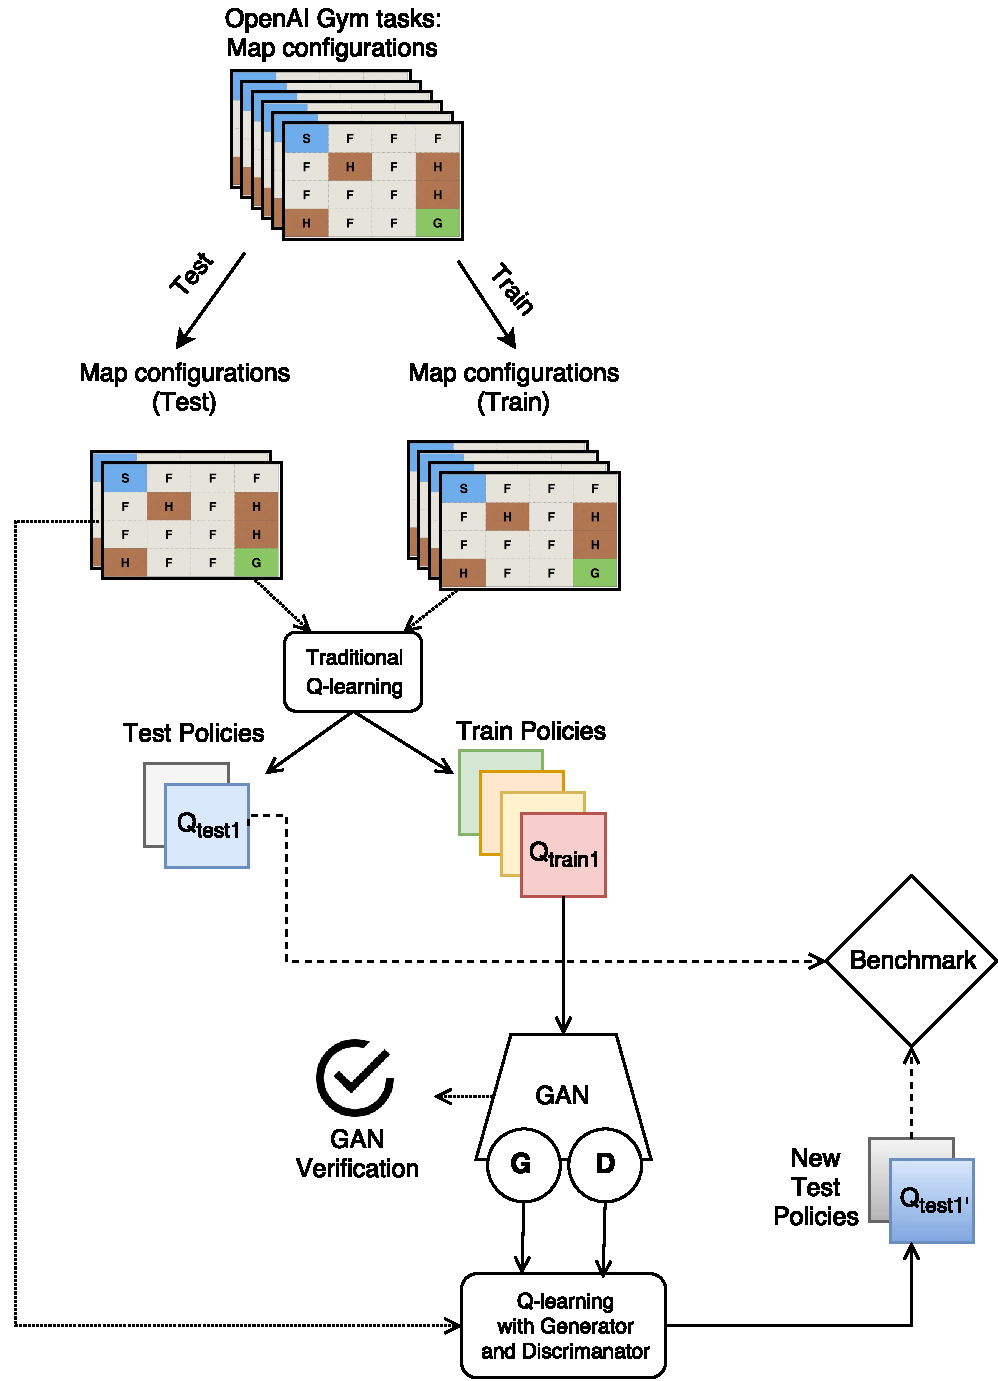
\includegraphics[width=10cm]{Figures/Pipeline}
\caption{The Data Pipeline}
\label{fig:pipeline}
\end{figure}

%----------------------------------------------------------------------------------------

\section{Structure of the report}
Our report is structured in a what that strongly follows each component of the data pipeline outlined in the previous subsection.
\begin{itemize}
	\item Chapter~\ref{Chapter2} introduces important background information on reinforcement learning, Markov Decision Processes, Q-learning and Generative Adversarial Networks.
	\item Chapter~\ref{Chapter3} details the environment being used in our experiments.
	\item Chapter~\ref{Chapter4} reports on the process of training policies on all the different tasks with traditional reinforcement learning (Q-learning).
	\item Chapter~\ref{Chapter5} outlines the process of training the GAN given the trained policies in the training set.
	\item Chapter~\ref{Chapter6} describes the new algorithm we develop to speed up learning on unseen tasks.
	\item Chapter
\end{itemize}

%----------------------------------------------------------------------------------------

\section{Main contributions}
% TODO:


%----------------------------------------------------------------------------------------